\section{Que es \texttt{checkinstall} y para que sirve?}

\texttt{checkinstall} es una utilidad que reemplaza temporalmente a la invocacion tradicional de \texttt{make install}.  
Su proposito principal es \textbf{generar un paquete binario} (DEB, RPM o TGZ, segun la distribucion) a partir de la instalacion que normalmente realizaria un script \texttt{Makefile}.  
En lugar de copiar archivos directamente al sistema de archivos, \texttt{checkinstall} intercepta el proceso, registra todos los archivos instalados y crea un paquete nativo:

\begin{itemize}[nosep]
  \item \textbf{Trazabilidad:} mantiene un registro exacto de los archivos instalados, lo que permite una desinstalacion limpia mediante el gestor de paquetes.
  \item \textbf{Consistencia:} integra el software compilado manualmente dentro de la base de datos de paquetes de la distribucion, evitando conflictos y archivos ``huerfanos''.
  \item \textbf{Portabilidad:} facilita distribuir el paquete a otros equipos con la misma distribucion sin recompilar.
\end{itemize}

\bigskip
Flujo simplificado de uso:

\begin{enumerate}[label=\arabic*.]
  \item \texttt{./configure \&\& make} \hfill (compila el proyecto)
  \item \texttt{sudo checkinstall --pkgname=mi-paquete --pkgversion=1.0} \hfill (intercepta \texttt{make install} y crea el .deb/.rpm)
  \item El paquete resultante aparece, por ejemplo, como \texttt{mi-paquete\_1.0-1\_amd64.deb}
  \item Instalacion normal con \texttt{sudo dpkg -i mi-paquete\_1.0-1\_amd64.deb}
\end{enumerate}

\newpage

%---------------------------------------------------------
\section{Empaquetar un ``Hello World'' con \texttt{checkinstall}}

A continuacion se muestra un ejemplo paso a paso para empaquetar un programa \emph{hello world} en~C:

\subsection*{1. Codigo fuente}

\begin{lstlisting}[language=C, caption={Archivo \texttt{hello.c}}]
#include <stdio.h>

int main(void) {
    puts("Hello World!");
    return 0;
}
\end{lstlisting}

\subsection*{2. Makefile minimal}

\begin{lstlisting}[language=make, caption={Archivo \texttt{Makefile}}]
CC  := gcc
CFLAGS := -Wall -O2
TARGET := hello

all:
	$(CC) $(CFLAGS) hello.c -o $(TARGET)

install:
	install -Dm755 hello /usr/local/bin/hello

clean:
	$(RM) hello
\end{lstlisting}

\subsection*{3. Crear el paquete}

\begin{enumerate}[label=\alph*)]
  \item Compilar: \texttt{make}
  \item Ejecutar:  
\begin{lstlisting}
sudo checkinstall --pkgname=hello --pkgversion=1.0 \
  --maintainer="tu@email.com" --pakdir=. \
  --install=no
\end{lstlisting}
  \item \texttt{checkinstall} preguntara descripcion, categoria, dependencias, etc.  
  \item El resultado sera \texttt{hello\_1.0-1\_amd64.deb} (o equivalente RPM/TGZ segun distro).
  \item Instalar con \texttt{sudo dpkg -i hello\_1.0-1\_amd64.deb}
\end{enumerate}

\subsection*{4. Verificar}

\begin{lstlisting}
$ which hello
/usr/local/bin/hello
$ hello
Hello World!
$ dpkg -L hello | head
/.
/usr
/usr/local
/usr/local/bin
/usr/local/bin/hello
\end{lstlisting}

El paquete puede desinstalarse con \texttt{sudo apt remove hello} o \texttt{sudo dpkg -r hello}, asegurando limpieza total.

Nosotros usamos el modulo de GitLab, con los siguientes resultados

\begin{figure}[h!]
  \centering
  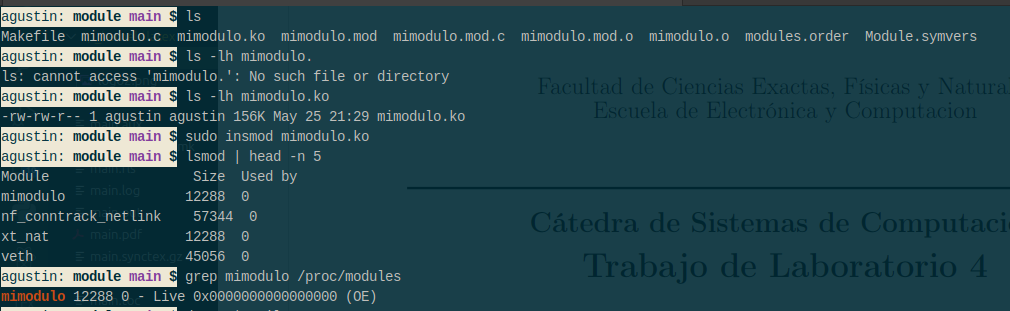
\includegraphics[width=0.8\linewidth]{images/paso1.png}
  \caption{Compilación y analisis del modulo.}
\end{figure}


\begin{figure}[h!]
  \centering
  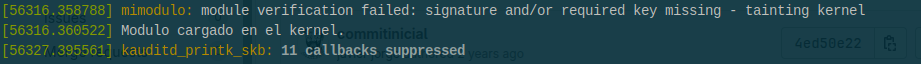
\includegraphics[width=0.8\linewidth]{images/kernellog.png}
  \caption{Log del kernel respecto al modulo propio.}
\end{figure}

\newpage

\section{Mejorar la seguridad del kernel: evitar modulos no firmados y mitigar rootkits}

Para fortalecer la seguridad del kernel es fundamental restringir la carga de modulos a aquellos que esten firmados y provenientes de fuentes confiables. A continuacion se enumeran acciones concretas respaldadas por la bibliografia consultada\footnote{Referencias: \emph{Linux Kernel Documentation: Kernel Lockdown}, \emph{Red Hat Secure Boot Guide}, \emph{The Art of Linux Kernel Design}.}:

\begin{enumerate}[label=\arabic*.]
  \item \textbf{Habilitar Secure Boot}: garantiza que el kernel y los modulos solo se carguen si estan firmados con claves de confianza (seccion~4).
  \item \textbf{Compilar el kernel con \texttt{CONFIG\_MODULE\_SIG\_FORCE=y}}: obliga a que cada modulo tenga firma valida; el kernel rechazara los no firmados.
  \item \textbf{Usar \texttt{module.sig\_enforce=1}} en la linea de comandos del kernel: equivalente en tiempo de arranque si el kernel ya se compilo con \texttt{CONFIG\_MODULE\_SIG}.
  \item \textbf{Implementar Lockdown Mode}: en kernels recientes (\texttt{CONFIG\_LOCKDOWN\_LSM}), opcionalmente activa restricciones adicionales que bloquean la manipulacion de memoria del kernel desde user space, incluso para \texttt{root}.
  \item \textbf{Activar SELinux/AppArmor perfiles estrictos}: reduce superficie de ataque para procesos potencialmente comprometidos que podrian intentar insertar modulos.
  \item \textbf{Deshabilitar \texttt{LOAD\_PIN\_ENFORCE}} (Lockdown PIN) solo si se requiere cargar modulos externos; de lo contrario, mantenerlo en enforcing.
  \item \textbf{Depurar modulos propios}: compilar con \texttt{-fstack\-protector\-strong}, \texttt{-D\_FORTIFY\_SOURCE=2}, habilitar CFI (\textit{Control Flow Integrity}) donde sea posible.
  \item \textbf{Monitorear firmas y blacklist}:
    \begin{itemize}[nosep]
      \item Revisar \texttt{/proc/sys/kernel/module\_sig\_enforce} (1 = obligatorio).
      \item Gestionar \texttt{.blacklist} del keyring para revocar claves comprometidas.
    \end{itemize}
  \item \textbf{Herramientas de deteccion de rootkits}: instalar y ejecutar periodicamente \texttt{rkhunter} y \texttt{chkrootkit}. Configurar alertas ante cambios en modulos del kernel o binarios criticos.
\end{enumerate}

Estas medidas, combinadas con un proceso de firmas propio (ver seccion de firma de modulos) y la generacion de paquetes reproducibles mediante herramientas como \texttt{checkinstall} o \texttt{dpkg-buildpackage}, minimizan el riesgo de rootkits que se basan en la insercion de modulos no autorizados.



